\chapter{Covolatility}\label{chap:covolatility}	 		% file "sect3.tex" 
Up to this stage, we have focussed on the volatility of a single series. We now turn to the task of estimating the correlation between two financial time series.  Volatility estimation plays an essential role since the volatilities of the component series appear in the denominator of the correlation calculation. However, estimation of the numerator presents a new problem because log-prices for the components are typically observed asynchronously, for example when using log-prices at the times of trades.

Not only did \citet{zhou1996high} suggest
how to estimate volatility, but remarkably he also suggested how to estimate covolatility with asynchronous data \citep{zhou1998estimating}. That is
important to note because much later, ten years later, Hayashi and Yoshida (HY) also came up with
a way of estimating covolatility. It turns out that Zhou had  discovered the HY estimator 
before HY did. One of our contributions in this chapter is to give recognition to
Zhou for his discovery before HY. We improve the HY estimate and come up with our
own correlation estimate. We show that this estimator has superior performance to the
Zhou-Hayashi-Yoshida estimate.

The  models in Chapter \ref{chap:volatility} can  be extended to multivariate asset processes in a straightforward manner. However there are complications in calculating cross-correlations between assets when the assets are traded asynchronously.  Nevertheless under certain conditions it is possible to estimate cross-correlations efficiently. We review methods that have been proposed over the last 20 years and identify key contributions.  We pay particular attention to a neglected paper by \citet{zhou1998estimating} and show that it contains essential ideas that generalise and pre-date more recent work. Our search for recursively defined estimators of covolatility that can be used in real-time high-frequency trading lead us to further generalisations of Zhou's estimator. Properties of the estimator are discussed and its variance is derived when working in tick time with constant parameters. In a simulation study the estimator is shown to outperform the popular covolatility estimator of \citet{hayashi2005covariance}. The chapter concludes with a discussion of the effectiveness of quasi-MLE methods with optimisation based on the Kalman filter and the use of an EM algorithm for asynchronous episodes.    

\section{Background}
The analysis of multivariate data is a central concern of financial management, not least in portfolio design where the objective is to exploit correlations between price movements of portfolio components to minimise risk. In high-frequency trading, short term correlations between assets can be exploited in the design of fast aggressive trading strategies and in the rapid defence of market making positions. 

In the theoretical financial literature, joint movements of log-returns of multiple assets are often modelled by correlated Brownian motion. Under the assumption that all of the assets are priced synchronously (in practice an unrealistic requirement) correlations and covariances can then be recovered from their realised versions. The procedures are described in \citet{barndorff2004econometric} along with the derivation of various limit theorems for the associated estimators.

There are various ways of dealing with asynchronous data. The simplest is to impose a common grid of `observation' times for all the assets involved and then to interpolate prices for each of the assets at these grid points. In an early study, \citet{epps1979comovements} showed that correlations obtained by this method depend on the size of the spacing, $h$, between the grid points. With the data that he had available, he found that the correlation reduced as $h \to 0$.  This has become known as the \emph{Epps effect}. A possible explanation in terms of persistent lag-correlation has been put forward by \citet{toth2009accurate,toth2009epps} but as \citet{zhou1998estimating} and others have noted, the effect can be explained simply by supposing that observations of the efficient log-price are contaminated by independent random noise.  As the sampling frequency increases, i.e.\ as $h \to 0$, returns are dominate by uncorrelated noise.  

For data derived from the `fighting screens' described by Zhou where promotional foreign exchange quotes are posted erratically on the Reuters screens, this may be an adequate explanations. For high-frequency exchange-traded assets in a modern trading environment more elaborate models are required, since observations of prices and volumes for quotes and trades are available more or less continuously with microsecond time resolution.  Nevertheless considerable theoretical research has been devoted to the  `efficient log-price plus noise' model and the model is usually accepted as a starting point for analysis. In this context, major contributions have been made by \citet{zhang2011estimating} using subsampling methods, extending similar work on volatility estimation. \citet{barndorff2011multivariate} show that kernel-based methods are closely related. In their work they advocate synchronising the processes at `renewal points', i.e.\ the succession of epochs at which a fresh price has been recorded for each of the assets. The most recent price for each asset is then used in correlation calculations.  They argue that the neglected `stale' prices contribute relatively little to the precision of covariance estimation. Their method has the advantage of providing non-negative definite estimates of the covariance matrix.  Their theoretical results and simulation studies are based on a flexible class of SDE based stochastic volatility models. Another recent and intuitively attractive approach, achieving comparable efficiency, is that of \emph{pre-averaging} where prices are smoothed over a rolling window before calculating cross-correlations \citep{jacod2009microstructure,podolskij2009estimation}.  

\citet{hayashi2005covariance} and earlier \citet{zhou1998estimating} take a different approach; the work of \citet{de1997high} is related. They use asynchronous data directly to obtain unbiased covariance estimators by summing cross-products of overlapping returns. Zhou shows that the estimator remains unbiased when there is observation noise and introduces a subsampling technique to deal with the consequential loss of precision. Zhou argues
there is an optimal sampling frequency. He is then able to provide guidance on the optimal choice of sampling frequency. In particular he is able to show infill consistency when observation error is negligible and the sampling frequency increases. The cross-product estimators of Zhou, Hayashi and Yoshida are the main focus of this chapter primarily because their linear structure can be exploited to provide a recursive estimator of covolatility that can be rapidly updated for high-frequency trading. The necessary modifications are described in Section \ref{sec:HYrecursion}.    

\section{Zhou-Hayashi-Yoshida estimators}\label{sec:cross}
Suppose we have two assets $A$ and $B$.  The log-price of $A$ is observed at discrete times $t \in \mathcal{T}$ and the log-price of $B$ at discrete times $u \in \mathcal{U}$.  For simplicity, we assume that a single `price' is provided at the given time points, for example the logarithm of the geometric mean of the bid and ask prices, or the regular mid-price.  The clock can run on physical time or some variant of tick time (TTS), for example the cumulative combined count of ticks for assets $A$ and $B$.  Both $\mathcal{T}$ and $\mathcal{U}$ will usually be irregularly spaced and the intersection $\mathcal{T} \cap \mathcal{U}$ may be empty. 

Let $\bX(t)$ and $\bY(u)$ be the latent efficient log-prices of assets $A$ and $B$, respectively, at given time points. In their initial analyses \citet{zhou1998estimating} and \citet{hayashi2005covariance} assume that the pair of log-prices $(\bX,\bY)$ is bivariate driftless Brownian motion with infinitesimal variances $\sigma^2_1(t)$ and $\sigma_2^2(t)$. In other words 
\begin{align}\label{eq:bivariateBM}
d\bX(t) &= \sigma_1(t) dB_1(t) \nonumber \\
d\bY(t) &= \sigma_2(t) dB_2(t),
\end{align}
where $B_1,B_2$ are correlated Brownian motions with $ \langle dB_1,dB_2\rangle = \rho(t)dt.$
  
At the first stage \citet{zhou1998estimating} and \citet{hayashi2005covariance} assume the log-prices can be observed without noise in an observation window $[0,1]$ with increasing sequences of observation times 
$\mathcal{T} = (t_0,\dots,t_{m})$ and
$\mathcal{U} = (u_0,\dots,u_{n})$,
where $t_0 = u_0 = 0$ and $t_{m} = u_{n} = 1$. Observation times are independent of the price process. 

Their objective is to estimate 
$$ c = \int_0^1 \sigma_{12}(t) dt,\quad \text{where} \quad  \sigma_{12}(t) = \sigma_1(t) \sigma_2(t)\rho(t).
$$
Their estimators are defined as follows.
%
\subsection{Definitions}\label{sec:ZHYdefns}
Let
\begin{eqnarray*}
R_i&=&\bX(t_i) - \bX(t_{i-1}),\;  i= 1,\dots,m \\
S_j&=&\bY(u_j) - \bY(u_{j-1}),\;  j= 1,\dots,n,
\end{eqnarray*}
be the returns of the latent log-prices of assets $A$ and $B$, respectively.

Let $J^X_i$ be the $i$th interval of time $(t_{i-1},t_i]$ for asset $A$ and let $\tau^X_i$ be the length of this return period. Similarly, let $J^Y_j = (u_{j-1},u_j]$ and $\tau^Y_j$ be the length of $J^Y_j$.

Now define $\tau_{ij}$ to be the length of the intersection between $J^X_i$ and $J^Y_j$, i.e.\ $\tau_{ij}$ is the length of time that the $i$th return period of asset $A$ and the $j$th return period of asset $B$ have in common.  This length could of course be zero.

Furthermore, let
\begin{eqnarray*}
t^+_j &= \min\{t_i,t_i \geqslant u_j\},\\
t^-_j &= \max\{t_i,t_i \leqslant u_j\},
\end{eqnarray*}
and 
\begin{eqnarray*}
u^+_i &= \min\{u_j,u_j \geqslant t_i\},\\
u^-_i &= \max\{u_j,u_j \leqslant t_i\},
\end{eqnarray*}
so that $t^+_j$ is the smallest time in $\mathcal{T}$ that is larger than or equal to $u_j$ and $t^-_j$ is the largest time in $\mathcal{T}$ that is smaller than or equal to $u_j$ and similarly for $u^+_i$  and $u^+_i$. 

Zhou's estimator is
\begin{equation}\label{eq:basicZhou}
\text{\rm Z} = \sum_{j=1}^{n} (\bX(t^+_j) - \bX(t^-_{j-1}))(\bY(u_j) - \bY(u_{j-1})).
\end{equation} 

Each term in \eqref{eq:basicZhou} is a product of returns. See Figure \ref{fig:overlapreturns}.
\begin{figure}[ht]
\centering
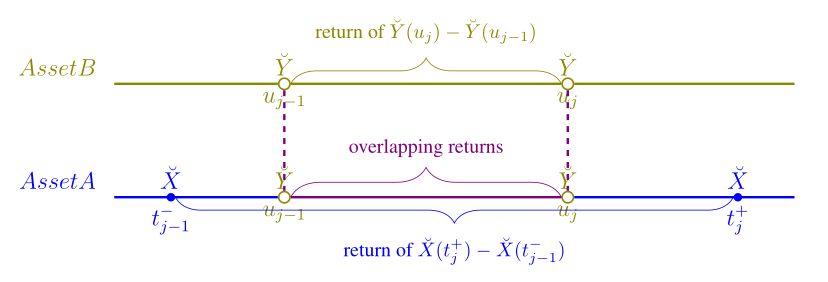
\includegraphics[width=\linewidth]{./Figures/overlapreturn.png} 
\caption{Illustration of the contribution of  terms in \eqref{eq:basicZhou}. The interval $(t^-_{j-1},t^+_j)$ contains $(u_{j-1},u_{j}).$}
	\label{fig:overlapreturns}
\end{figure}
%

Zhou's covariance estimate only involves return periods that \emph{overlap} since $X(t^+_j) - X(t^-_{j-1})$ can be written as contributions from three \emph{disjoint} intervals I, II, III as shown in Figure \ref{fig:zhoucov}. 
	$$\bX(t^+_j) - \bX(t^-_{j-1}) = (\bX(t^+_j) - \bX(u_j))+ (\bX(u_j) - \bX(u_{j-1}))+ (\bX(u_{j-1})- \bX(t^-_{j-1}))$$

\begin{figure}[h] 
\centering
    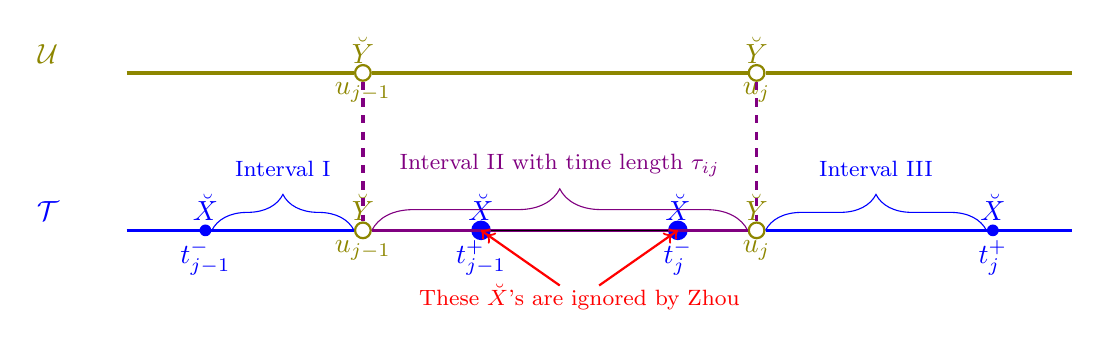
\begin{tikzpicture}[baseline=0pt]
    		% Draw four filled circles for points and define them as Tikz nodes of the 2nd line
    		\node [blue] (x1) at (1,0) [fill, circle,inner sep=1.5pt]{}  ;
    		\node [olive, thick] (y1) at (3,0) [draw, circle,inner sep=2pt]{};
    		    		%draw the middle 2 X's on the 2nd line
    		    		\node [blue] (xx1) at (4.5,0) [fill, circle,inner sep=2.5pt]{}  ;
    		    		\node [blue] (xx2) at (7,0) [fill, circle,inner sep=2.5pt]{}  ;  		 		
    		\node [olive, thick] (y2) at (8,0) [draw, circle,inner sep=2pt]{};
    		\node [blue] (x2) at (11,0) [fill, circle,inner sep=1.5pt]{};
    		% Label the points below the 2nd line
    		\draw (x1) node [below, blue] {$t^-_{j-1}$} 
			    	 	(y1) node [below, olive] {$u_{j-1}$}
    		    		    		(xx1) node [below, blue] {$t^+_{j-1}$} 
    		    		    		(xx2) node [below, blue] {$t^-_{j}$} 
    		(y2) node [below, olive] {$u_j$}
    		(x2) node [below, blue] {$t^+_{j}$} ;
    		% Label the points above the 2nd line       		
    		\draw (x1) node [above, blue] {$\breve{X}$} 
    		(y1) node [above, olive] {$\breve{Y}$}
    		    		    		(xx1) node [above, blue] {$\breve{X}$} 
    		    		    		(xx2) node [above, blue] {$\breve{X}$}   
    		(y2) node [above, olive] {$\breve{Y}$}
    		(x2) node [above, blue] {$\breve{X}$} ;
    		 %joint the points on the 2nd line
    		\draw [line width=1.2pt] [blue] (0,0) to (y1) 
    		(y2) to  (12,0);
    		\draw [line width=1.2pt] [violet] (y1) to  (y2);
    		    		
    		% Draw four filled circles for points and define them as Tikz nodes of the 1st line
    		\node [olive, thick] (yy1) at (3,2) [draw, circle,inner sep=2pt]{};
    		\node [olive, thick] (yy2) at (8,2) [draw, circle,inner sep=2pt]{};
    		\draw  (yy1) node [below, olive] {$u_{j-1}$}
    		(yy2) node [below, olive] {$u_j$}; 
    		\draw  (yy1) node [above, olive] {$\breve{Y}$}
    		(yy2) node [above, olive] {$\breve{Y}$}; 
    		%draw lines to joint the dots of the 1st line
    		\draw [line width=1.2pt] [olive] (yy1) to (yy2) 
    		(0,2) to (yy1)
    		(yy2) to (12,2);
			 %draw vertical line to joint the dots of Y's
    		\draw [line width=1.2pt] [violet] [dashed] (yy1) to (y1) 
    		(yy2) to (y2) ; 
			%draw the brace on the 2nd line lable it as  Interval I, II, III 
    		\draw [blue,decorate,decoration={brace,amplitude=13pt},] (x1)  -- (y1) 
    		node [blue,midway,above=16pt] {\footnotesize  Interval I};
    		\draw [violet,decorate,decoration={brace,amplitude=15pt},] (y1)  -- (y2) 
    		node [violet,midway,above=16pt] {\footnotesize   Interval II with time length $\tau_{ij}$ };
    		\draw [blue,decorate,decoration={brace,amplitude=13pt},xshift=0.4pt,yshift=-0.4pt] (y2)  -- (x2) 
    		node [blue,midway,above=16pt] {\footnotesize  Interval III }; 		
    		%label the axis as T and U on the left
	    	\draw[xshift=-1cm] [blue] (0,0) coordinate[label=above: $\mathcal{T}$]; 
			\draw[xshift=-1cm] [olive] (0,2) coordinate[label=above: $\mathcal{U}$]; 
    		%draw the arrows to point the 2 X's that Zhou ignores
    		\draw [<<-, thick] [red] (4.5, 0) -- (5.5,-0.7);
    		\draw [<<-, thick] [red] (7, 0) -- (6,-0.7);
    		\draw  (xx1)  -- (xx2) 	
    	    %lable the arrows to point the 2 X's that Zhou ignores
    		node [red,midway,below=16pt] {\footnotesize  These $\breve{X}$'s are ignored by Zhou};
    		
    		\end{tikzpicture}
    %	}
    	\caption{Zhou ignores some returns if there were events $\bX$ between the $\bY$ observations.}
    	\label{fig:zhoucov}
\end{figure}
    	
Zhou notes that his estimator can be expressed alternatively as 
$$\sum_{i=1}^{m} (\bX(t_i) - \bX(t_{i-1}))(\bY(u^+_i) - \bY(u^-_i)).$$
The estimator of \citet{hayashi2005covariance} is
\begin{equation}\label{eq:HY}
\text{\rm HY} = \sum_{i=1}^{m} \sum_{j=1}^{n} R_i S_j \mathbb{I}(\tau_{ij} >0).
\end{equation}

\citet{hayashi2005covariance} take \emph{every} return there is in the $A$ process and all the returns in the $B$ process: $R_i$'s and $ S_j $, but only multiply them together if there is an intersection between the return period, i.e.\ taking the product for every return period of $\bX$ process and the return period of $\bY$ process, with the indicator 0 if the intersection of the return periods is empty and 1, otherwise. See Figure \ref{fig:hycov}

\begin{figure}[h] 
	\centering
	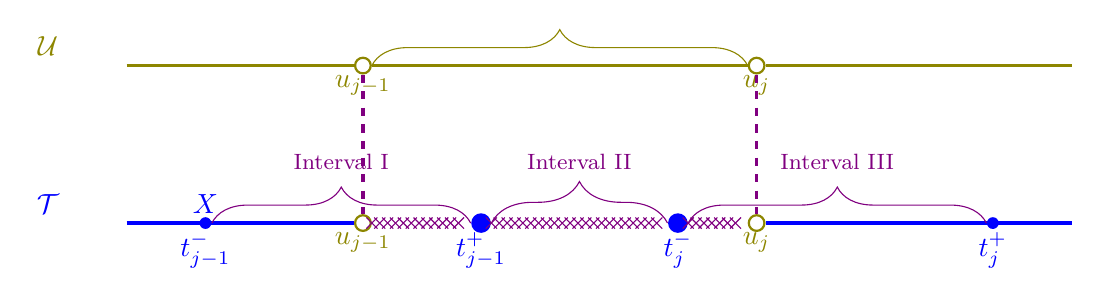
\begin{tikzpicture}

	    		% Draw four filled circles for points and define them as Tikz nodes of the 2nd line
	    		\node [blue] (x1) at (1,0) [fill, circle,inner sep=1.5pt]{}  ;
	    		\node [olive, thick] (y1) at (3,0) [draw, circle,inner sep=2pt]{};
	    		%draw the middle 2 X's on the 2nd line
	    		\node [blue] (xx1) at (4.5,0) [fill, circle,inner sep=2.5pt]{}  ;
	    		\node [blue] (xx2) at (7,0) [fill, circle,inner sep=2.5pt]{}  ;  		 		
	    		\node [olive, thick] (y2) at (8,0) [draw, circle,inner sep=2pt]{};
	    		\node [blue] (x2) at (11,0) [fill, circle,inner sep=1.5pt]{};
	    		% Label the points below the 2nd line
	    		\draw (x1) node [below, blue] {$t^-_{j-1}$} 
	    		(y1) node [below, olive] {$u_{j-1}$}
	    		(xx1) node [below, blue] {$t^+_{j-1}$} 
	    		(xx2) node [below, blue] {$t^-_{j}$} 
	    		(y2) node [below, olive] {$u_j$}
	    		(x2) node [below, blue] {$t^+_{j}$} ;
	    		% Label the points above the 2nd line       		
	    		\draw (x1) node [above, blue] {$X$} 
	    		(y1) node [above, olive] {$\bY$}
	    		(xx1) node [above, blue] {$\bX$} 
	    		(xx2) node [above, blue] {$\bX$}   
	    		(y2) node [above, olive] {$\bY$}
	    		(x2) node [above, blue] {$\bX$} ;
	    		
		 %joint the points on the 2nd line
	\draw [line width=1.2pt] [blue] (0,0) to (y1) 
	(y2) to  (12,0);
	(xx2) to  (yy2);
	%highlight the intersections
	 \draw [violet] decorate [decoration={border,angle=135,
	 	amplitude=0.1cm,segment length=1mm}]{(y1) to (xx1)};
	 	 \draw [violet] decorate [decoration={border,angle=45,
	 	 	amplitude=0.1cm,segment length=1mm}]{(y1) to (xx1)};
	 	 	 \draw [violet] decorate [decoration={border,angle=135,
	 	 	 	amplitude=0.1cm,segment length=1mm, mirror}]{(y1) to (xx1)};
	 	 	 \draw [violet] decorate [decoration={border,angle=45,
	 	 	 	amplitude=0.1cm,segment length=1mm,mirror}]{(y1) to (xx1)};
	
		 \draw [violet] decorate [decoration={border,angle=135,
		 	amplitude=0.1cm,segment length=1mm}]{(xx2) to (y2)};
		 \draw [violet] decorate [decoration={border,angle=45,
		 	amplitude=0.1cm,segment length=1mm}]{(xx2) to (y2)};
		 \draw [violet] decorate [decoration={border,angle=135,
		 	amplitude=0.1cm,segment length=1mm, mirror}]{(xx2) to (y2)};
		 \draw [violet] decorate [decoration={border,angle=45,
		 	amplitude=0.1cm,segment length=1mm,mirror}]{(xx2) to (y2)}; 	 		 
		 	
		 	\draw [violet] decorate [decoration={border,angle=135,
		 		amplitude=0.1cm,segment length=1mm}]{(xx1) to (xx2)};
		 	\draw [violet] decorate [decoration={border,angle=45,
		 		amplitude=0.1cm,segment length=1mm}]{(xx1) to (xx2)};
		 			 \draw [violet] decorate [decoration={border,angle=135,
		 			 	amplitude=0.1cm,segment length=1mm, mirror}]{(xx1) to (xx2)};
		 			 \draw [violet] decorate [decoration={border,angle=45,
		 			 	amplitude=0.1cm,segment length=1mm,mirror}]{(xx1) to (xx2)}; 
 
	     		    		%label the axis as T and U on the left
	     		\draw[xshift=-1cm] [blue] (0,0) coordinate[label=above: $\mathcal{T}$]; 
	     		\draw[xshift=-1cm] [olive] (0,2) coordinate[label=above: $\mathcal{U}$]; 

	%%%%%%%%%%%%%%%%%%%%%%%%

	    		% Draw four filled circles for points and define them as Tikz nodes of the 1st line
	    		\node [olive, thick] (yy1) at (3,2) [draw, circle,inner sep=2pt]{};
	    		\node [olive, thick] (yy2) at (8,2) [draw, circle,inner sep=2pt]{};
	    		\draw  (yy1) node [below, olive] {$u_{j-1}$}
	    		(yy2) node [below, olive] {$u_j$}; 
	    		\draw  (yy1) node [above, olive] {$\bY$}
	    		(yy2) node [above, olive] {$\bY$}; 
	    		%draw lines to joint the dots of the 1st line
	    		\draw [line width=1.2pt] [olive] (yy1) to (yy2) 
	    		(0,2) to (yy1)
	    		(yy2) to (12,2);
	    		%draw vertical line to joint the dots of Y's
	    		\draw [line width=1.2pt] [violet] [dashed] (yy1) to (y1) 
	    		(yy2) to (y2) ; 
	    		%draw the brace on the 1st line 
	
		\draw [olive,decorate,decoration={brace,amplitude=13pt}] (yy1)  -- (yy2) 
			node [olive,midway,below=16pt] {\footnotesize  };
				%draw the brace on the 2nd line lable it as  Interval I, II, III 				

		\draw [violet,decorate,decoration={brace,amplitude=13pt},] (x1)  -- (xx1) 
			node [violet,midway,above=16pt] {\footnotesize Interval I};
					\draw [violet,decorate,decoration={brace,amplitude=15pt},] (xx1)  -- (xx2) 			
					node [violet,midway,above=16pt] {\footnotesize Interval II  };
					\draw [violet,decorate,decoration={brace,amplitude=13pt},] (xx2)  -- (x2) 
					node [violet,midway,above=16pt] {\footnotesize Interval III };
	\end{tikzpicture}
	\caption{\citet{hayashi2005covariance} covariance estimator approach.}
	\label{fig:hycov}
\end{figure}

\subsection{Equivalence of Zhou and Hayashi-Yoshida estimators}
We claim the estimators are the same. This is straightforward since \eqref{eq:basicZhou} can be rewritten
as 
\begin{equation}\label{eq:ZhouHY} \sum_{j=1}^{n} (\bX(t^+_j) - \bX(t^-_{j-1}))S_j
\end{equation} and 
$$ \bX(t^+_j) - \bX(t^-_{j-1}) = \sum_{i=1}^{n} R_i \mathbb{I}(\tau_{ij} > 0).$$ There is a similar reduction for the second form of Zhou's estimator. Since the estimators are the same, from now on we will refer to this as the ZHY estimator. 
\paragraph{Unbiasedness:}
Under the above assumptions the ZHY estimator is unbiased for $c$. This follows from \eqref{eq:ZhouHY}. Writing
$R^{+}_j = \bX(t^+_j) - \bX(t^-_{j-1})$ for notational convenient, we note that 
$S_j$ is the return of $\bY$ over the interval $(u_{j-1},u_j]$ and $R^+_j$ is the return of $\bX$ over an interval that contains $(u_{j-1},u_j]$, so that 
$$R^+_j = \left[\bX(t^+_j) - \bX(u_{j})\right] + \left[\bX(u_{j}) - \bX(u_{j-1})\right] + \left[\bX(u_{j-1}) -  \bX(t^-_{j-1})\right].
$$
From the basic property of bivariate Brownian motion, the first and last bracketed terms are independent of $S_j$ and 
$$ \EE (\bX(u_{j}) - \bX(u_{j-1})) S_j  = \EE (\bX(u_{j}) - \bX(u_{j-1})) (\bY(u_{j}) - \bY(u_{j-1})) = \int_{u_{j-1}}^{u_j} \sigma_{12}(s) ds. $$ The unbiasedness then follows by summing over $j$. Both \citet{zhou1998estimating} and \citet{hayashi2005covariance} show that the ZHY estimator \emph{based on the latent efficient log-price} is infill consistent as the density of the observation points tends to infinity.

\subsection{Observation noise}

The ZHY estimator remains unbiased when subject to independent observation noise \citep{zhou1998estimating}, i.e.\ when
%
\begin{align}\label{eq:noiseAssumptions}
X(t_i) &= \breve{X}(t_i) + \epsilon_{i,1},\quad i = 0, \dots,m \notag\\
Y(u_j) &= \breve{Y}(u_j) + \epsilon_{j,2},\quad j = 0, \dots,n
\end{align}
%\end{array}
%\end{equation}
where $\breve{X}, \breve{Y}$ are latent bivariate Brownian log-prices and $\{\epsilon_{i,1}\}$,$\{\epsilon_{j,2}\}$ are independent mean zero sequences with variances $\eta_1^2$ and $\eta_2^2$, respectively. 

Although the ZHY estimator is unbiased, its variance is inflated -- as shown by  \citet{zhou1998estimating} who provides an approximation to the variance. By extending the techniques used in volatility estimation, \citet{zhang2011estimating} shows how to modify the ZHY estimator to provide infill consistency.
\subsection{Activity time -- constant parameters}\label{sec:HYrecursion}
For the remainder of this chapter we assume that the prices of both assets evolve on a common activity clock, such that the parameters $\sigma_1$, $\sigma_2$ and $\sigma_{12}$ are constant. A simple example could be the clock that counts the combined cumulative number of ticks of both assets.  In practice even with the best chosen clock, there will still be slow changes in the parameters and for this reason volatilities and covolatility are estimated in a moving window. As previously explained, there are speed advantages in expressing this as a recursive calculation.  

Since the ZHY estimator is linear in the time contributions, it lends itself to this type of modification.  For example, with the formulation \eqref{eq:basicZhou}, ZHY is replaced by
$$\text{ZHY}_m = \sum_{i=1}^{m} \wlambda^{m-i} (X(t_i) - X(t_{i-1}))(Y(u^+_i) - Y(u^-_i)), \quad 0 < \wlambda <1,$$  
so that $\text{ZHY}_m$ can be updated with the recursion
$$ \text{ZHY}_{m+1} = \wlambda \text{ZHY}_m + (X(t_{m+1}) - X(t_{m}))(Y(u^+_{m+1}) - Y(u^-_{m+1})).$$ 
In practice, traders will experiment with various values of $\wlambda$ to maximise the profitability of algorithms that depend on their covolatility estimator.

However, as we shall see the ZHY estimator is not the only linear estimator of $\sigma_{12}$ when this parameter is assumed to be constant. In the next section we introduce a general class of linear estimators and investigate their properties.      


\section{Extended ZHY estimator}\label{sec:extZHY}
We now propose an extension of the ZHY estimator in the form 
$$\sum_{i=1}^m \sum_{j=1}^n R_i S_j w_{ij} ,$$
where we introduce weighting factors $\{w_{ij}\}$ that are zero for non-intersecting return periods $J^X_i$ and $J^Y_j$. 

Note that the sum of products can be progressively updated as new data arrive, either in a moving window or recursively as described in Section \ref{sec:HYrecursion} -- an important consideration in online processing. 

Since 
$$ \EE\left(\sum_{i=1}^{m} \sum_{j=1}^{n} R_i S_j w_{ij}\right) = \sigma_{12} \sum_{i=1}^m \sum_{j=1}^n \tau_{ij} w_{ij}$$
it follows that the extended ZHY estimator  
\begin{equation}\label{eq:extendedZHY} 
\hat{\sigma}_{12} = \frac{\sum_{i=1}^{m}\sum_{j=1}^{n} R_i S_j w_{ij}\mathbb{I}(\tau_{ij} >0)}{\sum_{i=1}^{m} \sum_{j=1}^{n} \tau_{ij} w_{ij}}
\end{equation}
is unbiased for $\sigma_{12}$ (assumed constant).

The ZHY estimator is a special case where $w_{ij} = \mathbb{I}(\tau_{ij} > 0)$.
\subsection{Variance of the estimator} 
\begin{thm}\label{thm:genHY}
For given observation structure $\tau = \{\tau_{ij}\}$, under the assumptions of Section \ref{sec:cross} with constant $\sigma_1$,$\sigma_2$ and $\sigma_{12}$, the extended $\text{\rm ZHY}$ estimator has variance
$$\VV (\hat{\sigma}_{12}|\tau) = \sigma^2_1 \sigma^2_2 A_1 + \sigma^2_{12} A_2,$$
where 
\begin{equation}\label{eq:genZHY}
\begin{array}{lll}
A_1 &=& \left[\sum_{ij} w_{ij}^2 \tau_i^X \tau_j^Y \right] \bigg/\left(\sum_{ij} \tau_{ij} w_{ij}\right)^2 \\
A_2 &=& \left[\sum_i (\sum_j w_{ij} \tau_{ij})^2 + \sum_j(\sum_i w_{ij} \tau_{ij})^2 - \sum_{ij} w_{ij}^2 \tau_{ij}^2\right]\bigg/\left(\sum_{ij} \tau_{ij} w_{ij}\right)^2.
\end{array}
\end{equation}
\end{thm} 
\begin{proof}
The variance of $\sum_{i=1}^{m} \sum_{j=1}^{n} R_i S_j w_{ij}$ can be written as 
\begin{equation}\label{eq:varcov}
\sum_{ij} w_{ij}^2 \VV(R_i S_j) + \sum_{ij \neq kl}w_{ij} w_{kl} \CC(R_i S_j,R_k S_l),\end{equation}
and since
$$\left(\begin{array}{l} R_i\\S_j\\R_k\\S_l \end{array}\right) \sim N \left(0,\begin{array}{cccc}
\sigma^2_1 \tau_i^X & \sigma_{12} \tau_{ij} & 0 & \sigma_{12} \tau_{il} \\
\sigma_{12} \tau_{ij} & \sigma^2_2 \tau^Y_j & \sigma_{12} \tau_{kj} &0  \\
0 & \sigma_{12}\tau_{kj} & \sigma^2_1 \tau^X_{k} & \sigma_{12} \tau_{kl} \\
\sigma_{12} \tau_{il} & 0 & \sigma_{12} \tau_{kl} & \sigma^2_2 \tau^Y_l \end{array}
\right),
$$
we have 
\begin{eqnarray*}
\VV(R_i S_j) &=& \sigma^2_1 \sigma^2_2 \tau_i^X \tau_j^Y + \sigma_{12}^2 \tau^2_{ij} \\
\CC(R_i S_j, R_k S_l) &=& \tau_{il} \tau_{kj} \sigma^2_{12}, \quad ij \neq kl, 
\end{eqnarray*}
by standard distribution theory.

The first term in \eqref{eq:varcov}  reduces to 
$$ \sigma_1^2 \sigma_2^2 \sum_{ij} v^2_{ij} \tau_i^X \tau_j^Y + \sigma^2_{12}  \sum_{ij} v^2_{ij} \tau^2_{ij}.$$ 
The summation in second term of \eqref{eq:varcov} can be split into 3 cases
$$
\sum_{ij \neq kl} = \sum_{i=k,j \neq l} + \sum_{j=l,i \neq k} + \sum_{i \neq k, j \neq l}. $$
For the first case%, since $w_{ij} = w_{ij}$ when $\tau_{ij} > 0$, 
\begin{eqnarray*}
\sum_{i,j \neq l} w_{ij} w_{il} \CC(R_i S_j,R_k S_l) &=& \sigma^2_{12}\sum_{i,j \neq l} w_{ij} w_{il} \tau_{ij} \tau_{il} \\
& =&
\sigma^2_{12}\left[\sum_{i,j,l} w_{ij} w_{il} \tau_{ij} \tau_{il} - \sum_{ij} v^2_{ij} \tau^2_{ij}\right]\\
&=& 
\sigma^2_{12}\left[\sum_i(\sum_j w_{ij} \tau_{ij})^2  - \sum_{ij} v^2_{ij} \tau^2_{ij}\right],
\end{eqnarray*}
and similarly for the second case. 

For the third case, where $i \neq k$ and $j \neq l$, the summation becomes 
$$ 
\sigma^2_{12} \sum_{i \neq k, j \neq l} w_{ij} w_{kl} \tau_{il} \tau_{kj}.$$
But if $\tau_{il},\tau_{kj},w_{ij}$ and $w_{kl}$ are all non-zero then both $J^X_i$ and $J^X_k$ must intersect both $J^Y_j$ and $J^Y_l$ which is impossible since $J^X_i$ and $J^X_k$ are disjoint, as are $J^Y_j$ and $J^Y_l$. It follows that the summation in the third case is zero.

Collecting terms, the result follows.
\end{proof}

\begin{corollary}
\label{thm:basicHY}
Under the assumptions of Section \ref{sec:cross} the basic Zhou-Hayashi-Yoshida estimator has conditional variance
$$\VV (\text{\rm ZHY} | \tau) = \sigma^2_1 \sigma^2_2 B_1 + \sigma^2_{12} B_2,$$
where 
\begin{equation}\label{eq:varBasicHY}
\begin{array}{lll}
B_1 &=& \sum_{ij} \tau_i^X \tau_j^Y \mathbb{I}(\tau_{ij} >0)  \\ 
B_2 &=& \sum_i (\tau^X_i)^2 + \sum_j(\tau^Y_j)^2 - \sum_{ij} \tau_{ij}^2.
\end{array}
\end{equation}
\end{corollary} 
\begin{proof}
Noting that $\sum_{ij} \tau_{ij} = 1$, the total length of the interval $(0,1)$, and $\sum_i \tau_{ij} = \tau^X_j$ and $\sum_j \tau_{ij} = \tau^Y_i$, the result follows from \eqref{eq:genZHY}, by substituting $w_{ij} = \mathbb{I}(\tau_{ij} > 0)$.
\end{proof}

\section{A special  case}\label{sec:specialcase}
A special case of the extended estimator is got by replacing the returns $(R_i, S_j)$ in the basic ZHY estimator by interpolated versions reflecting the amount of overlap.  For asset $A$ the interpolated  value is $\tau_{ij} R_i/\tau^X_i$ and $\tau_{ij} S_j/\tau^Y_j$ for asset $B$. If the interpolated values are treated as actual log-returns then a natural estimator would involve the sum of their products divided by $\tau_{ij}$. The estimator then has the form
$$\sum_{i=1}^{m} \sum_{j=1}^{n}   R_i S_j \tau_{ij}/(\tau^X_i \tau^Y_j),$$
so that 
$$\tilde{\sigma}_{12} = \frac{\sum_{i=1}^{m} \sum_{j=1}^{n}  \tau_{ij} R_i S_j/(\tau^X_i \tau^Y_j) }{\sum_{i=1}^{m} \sum_{j=1}^{n} \tau^2_{ij}/(\tau^X_i \tau^Y_j)},$$ 
is an unbiased estimator of $\sigma_{12}$, with variance $\sigma^2_1 \sigma^2_2 C_1 + \sigma^2_{12} C_2,$
where 
\begin{align*}
C_1 &= 1/\sum_{ij} \theta_{ij}\\
C_2 &= \left[\sum_i (\sum_j \theta_{ij})^2 + \sum_j(\sum_i \theta_{ij})^2 - \sum_{ij} \theta_{ij}^2 \right]\bigg/\left(\sum_{ij} \theta_{ij} \right)^2,
\end{align*}
and $\theta_{ij} = \tau^2_{ij}/(\tau_i^X \tau^Y_j)$.
\subsection{Comparison with ZHY}\label{sec:noisefree}
The variances of ZHY and the new estimator $\tilde{\sigma}_{12}$ differ in the coefficients of $\sigma^2_1 \sigma^2_2$ and $\sigma^2_{12}$.  We can show that $C_1$ is never larger than $B_1$. To see this note that 
$$ \sum_{ij}\theta_{ij} = \sum_{ij} \tau_{ij} \mathbb{I}(\tau_{ij} > 0) \phi_{ij},$$
where $\sum_{ij}\tau_{ij} \mathbb{I}(\tau_{ij} > 0) = 1$ and $ \phi_{ij} = \tau_{ij}/(\tau_i^X \tau^Y_j.$  

In other words, $\sum_{ij}\theta_{ij}$ can be thought of as $\EE(\phi)$, the mean of $\phi_{ij}$ with the discrete probability mass function $\{p_{ij}\}$ where $p_{ij} = \tau_{ij} \mathbb{I}(\tau_{ij} > 0)$. 

By Jensen's inequality $\EE(1/\phi) \geqslant 1/\EE(\phi)$, so that
$$\sum_{ij} \frac{\tau_i^X \tau_j^Y}{\tau_{ij}} \tau_{ij} \mathbb{I}(\tau_{ij} > 0) \geqslant \left[
\sum_{ij} \frac{\tau_{ij}}{\tau_i^X \tau_j^Y} \tau_{ij} \mathbb{I}(\tau_{ij} > 0)\right]^{-1} = 1/\sum_{ij} \theta_{ij},$$
and $C_1 \leqslant B_1$ as claimed. 

The weights $w_{ij} = \tau_{ij}/(\tau^X_i \tau^Y_j)$ are in fact the optimal values as regards minimising $A_1$ in \eqref{eq:genZHY} for the general extended estimator.  This can be seen by considering the problem of minimising the numerator $ \sum_{ij} v^2_{ij} \tau^X_i \tau^Y_j \mathbb{I}(\tau_{ij}>0)$ with respect to $\{w_{ij}\}$ under the denominator constraint $\sum_{ij} \tau_{ij} w_{ij}$.  Introducing the Lagrange multiplier $\lambda$ and differentiating with respect to $w_{ij}$ we have
$$2 w_{ij} \tau^X_i \tau^Y_j + \lambda \tau_{ij} = 0,$$ so that
$$ w_{ij} \propto \tau_{ij} /(\tau^X_i \tau^Y_j).$$ 

Numerically we find $C_2$ is not always smaller than and $B_2$, but we can compare their average values and their empirical distributions when observation times are generated by Poisson processes, i.e.\ when $(t_1,\dots, t_m)$ and $(u_1, \dots, u_n)$ are associated with Poisson processes with rates $\lambda_1$ and $\lambda_2$, respectively.  
This is the approach adopted by \citet{hayashi2008asymptotic} in their asymptotic analysis of the ZHY estimator as $\lambda_1$ and $\lambda_2$ tend to infinity.  It is also the framework in which \citet{griffin2011covariance} compare the variance of the basic ZHY estimator with various estimators based on artificially synchronised prices. They derive expressions for the expected values of $B_1$ and $B_2$ valid for large values of $\lambda_1$ and $\lambda_2$.  These results can be also be derived directly from \eqref{eq:varBasicHY} by taking $M=m$ and $N=n$ to have Poisson distributions conditioned to be positive and $(t_1,\dots, t_{m})$ and $(u_1, \dots, u_{n})$  to be Poisson process event times conditional on $t_m = u_n  = 1$. 

For $\EE(B_2)$ we then have conditionally on $M=m$ and $N=n$
$$ \EE(B_2| m,n) = m \EE[(\tau_1^X)^2] + n \EE[(\tau^X_1)^2] - (m+n-1)\EE(\tau^2),$$
where $\tau_1^X$, $\tau_1^Y$ are typical values of $\tau_i^X$ and $\tau_j^Y$ and $\tau$ is a typical gap in the ordered union of $(t_1,\dots, t_m)$ and $(u_1, \dots, u_n)$.  

Since 
$$\PP(\tau_1^X > x|m) = (1-x)^{m-1}, \quad 0<x<1,$$
it follows that $\EE[(\tau_1^X)^2| m] = 2/[m(m+1)]$ so that unconditionally 
$$\EE[M (\tau_1^X)^2] = \sum_{m=1}^\infty \frac{2\; \text{e}^{-\lambda_1}\lambda^m_1}{ (m+1) m! (1 - \text{e}^{-\lambda_1})} =\frac{2}{\lambda_1} - \frac{2}{\text{e}^{\lambda_1} -1} \sim \frac{2}{\lambda_1}. $$  
Similarly, $\EE[(\tau_1^Y)^2] \sim 2/\lambda_2$ and $\EE[\tau^2] \sim 2/(\lambda_1+\lambda_2)$, so that
\begin{equation}\label{eq:expB2}\EE(B_2) \sim \frac{2}{\lambda_1} + \frac{2}{\lambda_2} - \frac{2}{\lambda_1 + \lambda_2},\end{equation}
as $\lambda_1$ and $\lambda_2$ tend to infinity. 

In the same way it can be shown that
\begin{equation}\label{eq:expB1}
\EE(B_1) \sim \frac{2}{\lambda_1} + \frac{2}{\lambda_2}.\end{equation}
in agreement with \citet{griffin2011covariance}. We have confirmed the result both algebraically and
numerically.

Note however that Griffin and Oomen give the value 
$$ \frac{2}{{\lambda_1 + \lambda_2}}\left(\frac{\lambda_1}{\lambda_2} + \frac{\lambda_2}{\lambda_1}\right)$$ for $\EE(B_2)$. This appears to be in error. We have confirmed this error both algebraically and numerically by simulation.

\subsection{Numerical comparisons}
From the general form of the variances we see it is only necessary to compare the coefficients of $\sigma^2_1 \sigma_2^2$ and $\sigma_{12}^2$ and that these only depend on the timestamp structure. 
We have shown that $C_1$ is never larger than $B_1$ however when $m+n$ is small we have found cases where $C_2$ is larger than $B_2$. These seem to be rare cases. To illustrate the typical relative performance of $\tilde{\sigma}_{12}$ and $ZHY$, we present numerical results working with timestamps from independent Poisson processes. 
Along the way, we were able to confirm the accuracy of \eqref{eq:expB1} and \eqref{eq:expB2}.
The results are presented in Figure \ref{fig:BC}. 
\begin{figure}[!ht]
\centering
  \begin{subfigure}[l]{0.49\textwidth}
    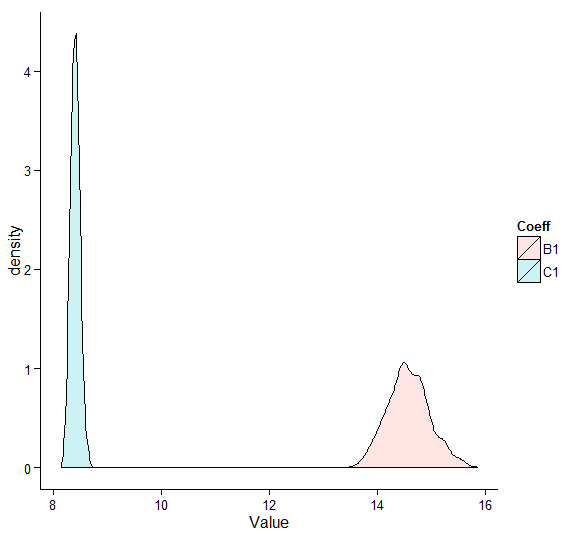
\includegraphics[width=\textwidth]{./Figures/BC1.png}
    \caption{}
    \label{fig:BCa}
  \end{subfigure} 
  \begin{subfigure}[l]{0.49\textwidth}
    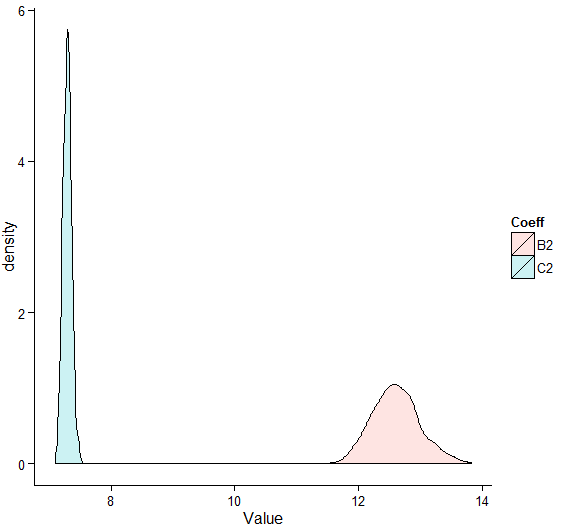
\includegraphics[width=\textwidth]{./Figures/BC2.png}
    \caption{}
    \label{fig:BCb}
  \end{subfigure}
  \begin{subfigure}[l]{\textwidth}
    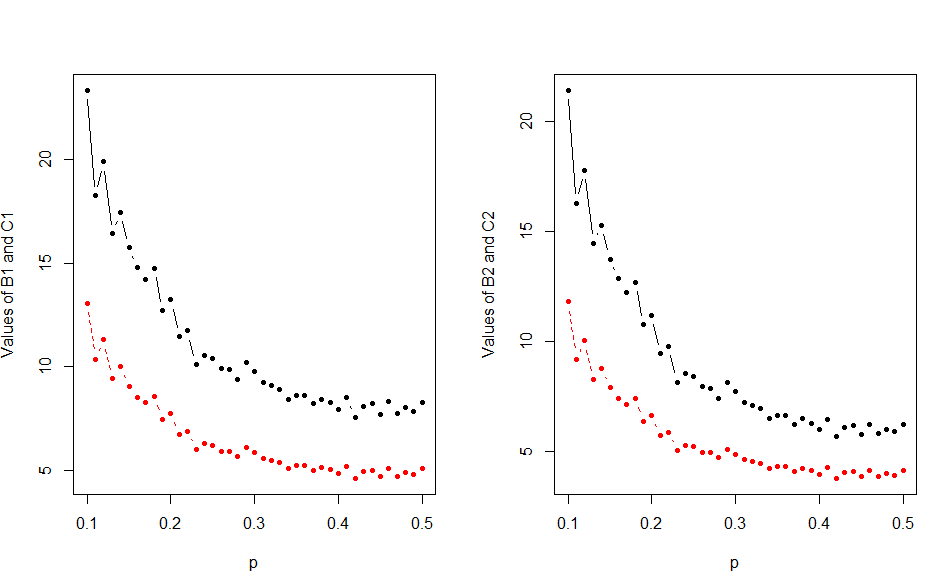
\includegraphics[width=\textwidth]{./Figures/extendedZHY.PNG}
    \caption{}
    \label{fig:BCc}
  \end{subfigure}
\caption{Panel (a) compares simulated values of $B_1$ and $C_1$. Panel (b) compares $B_2$ and $C_2$. In both cases there are 1000 simulations with $\lambda_1 = 1000$ and $\lambda_2 = 5000$ and the coefficients are scaled by $\lambda_1+\lambda_2$ for convenient axis values. Panel (c) shows the effect of varying the ratio $p = \lambda_1/(\lambda_1+\lambda_2)$. \label{fig:BC}}
\end{figure}

We see that in both cases the coefficients in the extended ZHY has are substantially smaller those for the standard ZHY estimator. We also compare the values of the coefficients for various value of the ratio $p = \lambda_1/(\lambda_1+\lambda_2)$ in Figure \ref{fig:BC}. 
Again the extended ZHY estimator is consistently better.    



 For completeness we will derive the exact variance for the general class of estimator proposed in Section \ref{sec:extZHY} as a function of the time-stamp structure. Some additional notation is required.

\subsection{Additional notation}
The time-stamp structure is determined by $(\mathcal{T},\mathcal{U})$, the two sequences of observation times between $0$ and $1$.  When these sequences are interleaved, the gaps in the combined sequence have lengths $\{\tau_{ij}\}$, where $\tau_{ij}$ is the length of the overlap between $\tau_i^X$ and $\tau^Y_j$.  Since $\mathcal{T} = (t_0,\dots,t_m)$ and $\mathcal{U} = (u_0,\dots,u_n)$, the number of these gaps is $L=m+n-1$. It is convenient to number the gaps as $p = 1,\dots,L$, from left to right, and then define  $w_{[p]}$ to be the value of $w_{ij}$ associated with the $p$th gap, $ p = 1,\dots,L$, i.e.\ the gap where $J^X_i$ and $J^Y_j$ overlap. For notational convenience we also put $w_{[0]} = w_{[N+1]} = 0$.

Since $w_{[p]}$ is associated with a gap in the combined sequence, it will either lie between timestamps that are both from $\mathcal{T}$, both from $\mathcal{U}$ or otherwise.  We denote the latter case where there is alternation, by $Q$
%, and define
%$$ D(v) =  \sum_{p \in Q} w_{[p-1]}w_{[p+1]}.$$
\begin{thm}\label{thm:genZHYnoise}
Under the assumptions \eqref{eq:noiseAssumptions}, with normally distributed observation error, the extended ZHY estimator has variance
$$\VV (\hat{\sigma}_{12}) = \sigma^2_1 \sigma^2_2 A_1 + \sigma^2_{12} A_2 + \big[\nu_1^2 \sigma^2_2 D_1 + \nu_2^2\sigma_1^2 D_2 + \nu_1^2 \nu_2^2 D_3\big]/T^2(v),$$
where 
\begin{align} %\label{eq:genZHYnoise}
A_1 &= \big[\sum_{ij} w_{ij}^2 \tau_i^X \tau_j^Y\big]/T^2(w)  \notag \\
A_2 &= \big[\sum_i (\sum_j w_{ij} \tau_{ij})^2 + \sum_j(\sum_i w_{ij} \tau_{ij})^2 - \sum_{ij} w_{ij}^2 \tau_{ij}^2\big]/T^2(w) \notag\\
D_1 &= 2 \sum_i \tau^X_i [\sum_j w_{ij}^2 - \sum_j w_{ij} w_{i,j+1}]\notag\\
D_2 &= 2 \sum_j \tau^Y_j [\sum_i w_{ij}^2 - \sum_i w_{ij} w_{i+1,j}]\notag\\
D_3 &= 4 \sum_{p=1}^{L-1} (w_{[p]} - w_{[p+1]})^2 + 2 \sum_{p \in Q} w_{[p-1]}w_{[p+1]}\notag\\
T(w)&= \sum_{ij} \tau_{ij} w_{ij}
\end{align}

\end{thm} 
\begin{proof}
From \eqref{eq:extendedZHY} the variance of $\hat{\sigma}_{12}$ is $\VV \big(\sum_{ij} R_i S_j w_{ij})/T^2(w)$, where 
\begin{equation}\label{eq:extVar} \VV \big(\sum_{ij} R_i S_j w_{ij}) = \sum_{ij} w_{ij}^2 \VV(R_i S_j\big) + \sum_{ij \neq kl}w_{ij} w_{kl} \CC(R_i S_j,R_k S_l).\end{equation}
By the assumptions of the theorem, the vector $(R_i,S_j,R_k,S_l)\tz$ is multivariate normal with
$$ \begin{array}{llll}
\VV(R_i) &= \sigma_1^2 \tau_i^X + 2 \nu_1^2 & \VV(R_k) &= \sigma_1^2 \tau_k^X + 2 \nu_1^2 \\
\VV(S_j) &= \sigma_2^2 \tau_j^Y + 2 \nu_2^2 & \VV(S_l) &= \sigma_2^2 \tau_l^Y + 2 \nu_2^2
\end{array}
$$
and  
$$ \begin{array}{llll}
\CC(R_i, S_j) &= \sigma_{12} \tau_{ij} & \CC(R_k, S_j) &= \sigma_{12} \tau_{kj} \\
\CC(R_i, S_l) &= \sigma_{12} \tau_{il} & \CC(R_k, S_l) &= \sigma_{12} \tau_{kl} \\
\CC(R_i, R_k) &= - \nu_1^2 \mathbb{I}_1(i \sim k) & \CC(S_j, S_l) &= - \nu_2^2 \mathbb{I}_2(j \sim l),
\end{array}
$$
where the indicator $\mathbb{I}_1(i \sim k)$ is $1$ when $J^X_i$ is adjacent to $J^X_k$ and similarly $\mathbb{I}_2(j \sim l) = 1$ when $J^Y_j$ is adjacent to $J^Y_l$. 

It follows again by standard normal distribution theory that  
$$
\begin{array}{rl}
\VV(R_i S_j) &= (\sigma_1^2 \tau_i^X + 2 \nu_1^2)(\sigma_2^2 \tau_j^Y + 2 \nu_2^2)\\
\CC(R_i S_j, R_i S_l) &= \sigma^2_{12}  \tau_{ij} \tau_{il} - \nu_2^2 \mathbb{I}_2(j \sim l) (\sigma_1^2 \tau_i^X  + 2 \nu_1^2), \quad j \neq l\\
\CC(R_i S_j, R_k S_j) &= \sigma^2_{12}  \tau_{ij} \tau_{kj} - \nu_1^2 \mathbb{I}I_1(i \sim k) (\sigma_2^2 \tau_j^Y  + 2 \nu_2^2), \quad i \neq k \\
\CC(R_i S_j, R_k S_l) &= \sigma^2_{12}  \tau_{il} \tau_{kl} + \nu_1^2 \nu_2^2 \mathbb{I}_1(i \sim k) \mathbb{I}_2(j\sim l), \quad i\neq k, j \neq l
\end{array}
$$
The first term on the right-hand side of \eqref{eq:extVar} reduces to 
\begin{align}\label{eq:varcase}
\sum_{ij} \VV(R_i S_j)w_{ij}^2 &= \sigma_1^2 \sigma_2^2 \sum_{ij} \tau_i^X \tau_j^Y v^2_{ij}
+2\nu_2^2 \sigma_1^2 \sum_i \tau_i^X \sum_j v^2_{ij} \notag \\
&+2\nu_1^2 \sigma_2^2 \sum_j \tau_j^Y \sum_i v^2_{ij}  
+4 \nu_1^2 \nu_2^2 \sum_{ij} v^2_{ij} .
\end{align} 

The second summation on the right-hand side of \eqref{eq:extVar} can be split into 3 cases
$$
\sum_{ij \neq kl} = \sum_{i=k,j \neq l} + \sum_{j=l,i \neq k} + \sum_{i \neq k, j \neq l}. $$
For the first case,
\begin{align}\label{eq:firstcase}
&\sum_{i=k,j \neq l} w_{ij} w_{il} \CC(R_i S_j,R_i S_l) \notag \\ 
&\quad = \sigma^2_{12}\sum_{i,j \neq l} w_{ij} w_{il} \tau_{ij} \tau_{il} - \nu_2^2\sum_{i,j \neq l} (\sigma_1^2 \tau_i^X + 2\nu_1^2) w_{ij} w_{il}  \mathbb{I}_2(j \sim l) \notag \\
&\quad= \sigma^2_{12}\big[\sum_i(\sum_j w_{ij} \tau_{ij})^2  - \sum_{ij} v^2_{ij} \tau^2_{ij}\big] - \nu_2^2\sum_i (\sigma_1^2 \tau_i^X + 2\nu_1^2) P_i^Y 
\end{align}
where $P^Y_i$ is the sum of products $w_{ij}w_{il}$ for all pairs $(j,l)$ such that $J_j^Y$ and $J_l^Y$ are adjacent, i.e.\ 
$P_i^Y =  2\sum_j w_{ij} w_{i,j+1}.$

Similarly for the second case 
\begin{align}\label{eq:secondcase}
&\sum_{j=l,i \neq k} w_{ij} w_{kj} \CC(R_i S_j,R_k S_j) \notag \\ 
&\quad=  \sigma^2_{12}\big[\sum_j(\sum_i w_{ij} \tau_{ij})^2  - \sum_{ij} v^2_{ij} \tau^2_{ij}\big] - \nu_1^2\sum_j (\sigma_2^2 \tau_j^Y + 2\nu_2^2) P_j^X, 
\end{align}
where $P^X_j$ is the sum of products $w_{ij}w_{kj}$ for all pairs $(i,k)$ such that $J_i^X$ and $J_k^X$ are adjacent, i.e.\ 
$P_j^X =  2\sum_i w_{ij} w_{i+1,j}.$

For the third case 
\begin{align}\label{eq:Allneighbours}
&\sum_{i \neq k, j \neq l} w_{ij} w_{kl} \CC(R_i S_j,R_k S_l) \notag \\ 
&\quad= \sum_{i \neq k, j \neq l} \sigma^2_{12} w_{ij} w_{kl} \tau_{il} \tau_{kj} + \nu_1^2 \nu_2^2 \sum_{i \neq k, j \neq l}w_{ij} w_{kl}\mathbb{I}_1(i \sim k) \mathbb{I}_2(j\sim l) \notag \\
&\quad= \quad 0 + \nu_1^2 \nu_2^2 \sum_{i \neq k, j \neq l}w_{ij} w_{kl}\mathbb{I}_1(i \sim k) \mathbb{I}_2(j\sim l),
\end{align}
since if $\tau_{il},\tau_{kj},w_{ij}$ and $w_{kl}$ are all non-zero then both $J^X_i$ and $J^X_k$ must intersect both $J^Y_j$ and $J^Y_l$ which is impossible since $J^X_i$ and $J^X_k$ are disjoint, as are $J^Y_j$ and $J^Y_l$. 

From \eqref{eq:Allneighbours}, referring to Figure \ref{fig:alternation}, 
we see that 
\begin{equation}\label{eq:lastcase}\sum_{i \neq k, j \neq l}w_{ij} w_{kl}\mathbb{I}_1(i \sim k) \mathbb{I}_2(j\sim l) =  2 \sum_{p \in Q} w_{[p-1]}w_{[p+1]},\end{equation}
since when $(J^X_i,J^X_k)$ and $(J^Y_j,J^Y_l)$ are both neighbouring pairs, the products $w_{ij} w_{kl}$ are non-zero unless there is an alternation at one of the gaps $\tau_{ij}$, $\tau_{il}$,$\tau_{kj}$ or $\tau_{kl}$. Furthermore there are only two such arrangements since the ordering $(i,k)$ has to agree with the ordering $(j,l)$.
\begin{figure}[!ht]
\centering
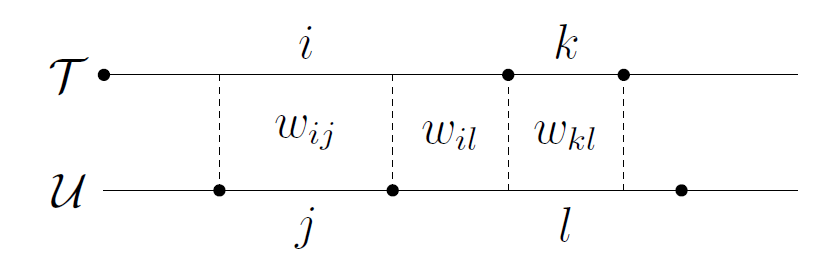
\includegraphics[width=0.7\linewidth]{./Figures/alternationV2.png}
\caption{An alternation between $\mathcal{T}$ and $\mathcal{U}$ timestamps at the gap $\tau_{il}$. The ordering $(i,k)$ has to agree with the ordering $(j,l)$ to have both $w_{ij}$ and $w_{kl}$ non-zero.\label{fig:alternation} }
\end{figure}

Collecting coefficients of $\sigma^2_1 \sigma^2_2$ and $\sigma_{12}^2$, the expressions for $A_1$ and $A_2$ follow as in Theorem \ref{thm:genHY}.  


The coefficient of $\nu_1^2 \sigma^2_2$ comes from \eqref{eq:firstcase} and \eqref{eq:varcase}. Similarly, the coefficient of $\nu_1^2 \sigma^2_2$ is from 
\eqref{eq:secondcase} and \eqref{eq:varcase}.  

Collecting terms in $\nu^2_1 \nu^2_2$ from \eqref{eq:varcase}, \eqref{eq:firstcase} and \eqref{eq:secondcase} we have
$$ 4 \sum_{ij} w_{ij}^2 - 4\sum_j w_{ij} w_{i,j+1} - 4\sum_i w_{ij} w_{i+1,j} = 4 \sum_p(w_{[p]} - w_{[p+1]})^2,$$
and together with \eqref{eq:lastcase} we have $D_3$.
\end{proof} 
There is simplification in the basic ZHY case where $w_{ij} = \mathbb{I}_{ij}$.
\begin{corollary}
\label{thm:basicHYNoise}
Under the assumptions of Theorem \ref{thm:genZHYnoise}, the basic Zhou-Hayashi-Yoshida estimator has conditional variance
$$\VV (\text{\rm ZHY} | \tau) = \sigma^2_1 \sigma^2_2 B_1 + \sigma^2_{12} B_2 + 2 \nu_1^2 \sigma^2_2 + 2 \nu_2^2 \sigma^2_1 + 4 \nu_1^2 \nu_2^2 |Q|,$$
where 
\begin{equation}\label{eq:varBasicHYnoise}
\begin{array}{lll}
B_1 &=& \sum_{ij} \tau_i^X \tau_j^Y \mathbb{I}(\tau_{ij} >0)  \\ 
B_2 &=& \sum_i (\tau^X_i)^2 + \sum_j(\tau^Y_j)^2 - \sum_{ij} \tau_{ij}^2,
\end{array}
\end{equation}
and $|Q|$ is the number of alternating gaps.
\end{corollary} 
\begin{proof}
For $B_1$ and $B_2$, the result follows as in Corollary \ref{thm:basicHY}; it also follows that $T(w) = 1$.  The coefficient of $\nu_1^2 \sigma_2^2$ can be obtained from $D_1$ in Theorem \ref{thm:genZHYnoise} with $w_{ij} = \mathbb{I}(\tau_{ij}>0)$. Note that $\sum_j \mathbb{I}(\tau_{ij}>0)$ is the number of $J_j^Y$ returns that overlap $J^X_i$ and  $\sum_j \mathbb{I}(\tau_{ij}>0)\mathbb{I}(\tau_{i,j+1}>0)$ is the number of timestamps in $\mathcal{U}$ that lie inside $J^X_i$, i.e.\ one fewer than the number of $J_j^Y$ returns that overlap $J^X_i$. It follows that 
$$\sum_j \mathbb{I}^2(\tau_{ij}>0) - \sum_j \mathbb{I}(\tau_{ij}>0) \mathbb{I}(\tau_{i,j+1}>0) = 1,$$ 
and similarly for   $D_2$. Finally, $w_{ij} = \mathbb{I}(\tau_{ij}>0)$ implies $w_{[p]} = 1, p=1,\dots,N$ so the first term in $D_3$ is zero and the second term is the number of alternations $|Q|$. 
\end{proof}
As in the noiseless case we can consider the average value of the variance when the timestamps are from two independent Poisson processes with rates $\lambda_1$ and $\lambda_2$, respectively. Beyond the noise free case discussed in Section \ref{sec:noisefree}, this only requires the evaluation of $\EE(|Q|)$. But the probability of an alternation is $2\alpha (1-\alpha)$ where $\alpha = \lambda_1/(\lambda_1 + \lambda_2)$, and since the expected number of gaps is of order $\lambda_1 + \lambda_2$, it follows that $\EE(|Q|) \sim \lambda_1 \lambda_2/(\lambda_1+\lambda_2)$, in agreement with the result obtained by \citet{griffin2011covariance}.

\subsection{Further extensions}
The estimators we have considered so far can be extended by \emph{subsampling}.  This was proposed originally by \citet{zhou1998estimating} and follows naturally from the subsampling methods that he proposed for volatility estimation in \citet{zhou1996high}.  The basic idea is use a sample of every $k$th observation to estimate the parameter and then to average the resulting values.  Zhou shows that this will reduce the standard error and he makes recommendations about the optimal value of $k$.  See also \citet{griffin2011covariance} and the references therein for recent applications of this technique.

\section{Maximum likelihood estimation}
We now look briefly at the problem of maximum likelihood estimation under strong model assumptions, specifically the case where the efficient price can be observed without noise and the infinitesimal parameters are constant. We note however, as before, that it may be possible to remove microstructure noise using the methods of \citet{robert2012volatility} and that we can also deal with time-varying parameters by suitable rescaling of time. 

When $(\breve{X},\breve{Y})$ is bivariate Brownian motion, as in Section \ref{eq:bivariateBM}, the likelihood of the observed value $\bar{r}$ of the combined vector of returns $\bar{R} = (R,S)$  is 
$$L(\theta) = \frac{\exp\left(-\frac12 \bar{r}^\text{\sf T} V^{-1} \bar{r}\right)}{(2 \pi)^{(m+n)/2}\sqrt{\text{det}(V)}},$$
where 
$$V = \left(\begin{array}{cc} \sigma^2_1 D_1& \sigma_{12} B\\ \sigma_{12} B^\text{T}&\sigma^2_2 D_2 \end{array}\right),$$
and
$$D_1 = \text{diag}(\tau_i^X; i=1,\dots,m), \quad   D_2 = \text{diag}(\tau_j^Y; j=1,\dots,n)$$ 
and $B$ is a matrix with elements $B_{ij}= \tau_{ij}; i=1,\dots,m; j=1,\dots,n $.

In principle, the parameters $\theta = (\sigma_{1},\sigma_{2},\sigma_{12})$ can then be estimated by maximum likelihood and the correlation recovered from
$$ \hat{\rho} = \frac{\hat{\sigma}_{12}}{\hat{\sigma}_1 \hat{\sigma}_2},$$
but the vector $\bar{r}$ is very long and it is computationally very expensive to obtain the maximum likelihood
estimate.
The EM algorithm offers a possible computational approach.
\subsection{EM algorithm}
We start by supposing that we have full synchronous data for both assets. In this case it is easy to find the MLE. Recall that to apply the EM algorithm we need to calculate the expected value of the full log-likelihood given our partially observed data \citep{dempster1977maximum}.

Suppose that we have synchronous price information for assets $A$ and asset $B$ at every time  $t \in  \mathcal{T} \cup \mathcal{U}$.  Let $\tilde{\tau}_1,\tilde{\tau}_2, \dots, \tilde{\tau}_L$ be the return times for the full data and denote the associated log-returns of the assets by $(\tilde{R}_k,\tilde{S}_k); k=1,2,\dots,L$.  In this case, we simply have a sequence of independent pairs. The $k$th pair has a bivariate normal distribution with mean zero and variance-covariance matrix $\tilde{\tau}_k\Sigma$.  

The full likelihood is then
$$\tilde{L}(\theta) = \frac{\exp\left[-\frac12(1-\rho^2)^{-1}\left(\sigma_{1}^{-2} h_{1,1}
 - 2 \rho (\sigma_{1} \sigma_{2})^{-1} h_{1,2} + \sigma_{2}^{-2} h_{2,2}\right)\right]}
 {(2 \pi \sigma_{1} \sigma_{2} (1-\rho^2)^{1/2})^N (\prod \tilde{\tau}_k)^{1/2}},$$
where 
$$ H_{1,1} = \sum_{k=1}^N \tilde{R}_k^2/\tilde{\tau}_k, \quad H_{1,2} = \sum_{k=1}^N \tilde{R}_k \tilde{S}_k /\tilde{\tau}_k,
 \quad \text{and}\quad H_{2,2} = \sum_{k=1}^N \tilde{S}_k^2 /\tilde{\tau}_k.$$

 
It is well-known, and straightforward to show, that the MLEs are
$$\tilde{\sigma}_1^2 = N^{-1} H_{1,1}, \quad \tilde{\sigma}_{12} = N^{-1} H_{1,2},\quad \tilde{\sigma}^2_2 = N^{-1} H_{2,2}$$ 
To apply the EM algorithm we need the expectation of $\log(\tilde{L}(\theta)$, in particular the expectations of $H_{1,1},H_{1,2}$ and $H_{2,2}$ given $\bar{R}=\bar{r}$, as follows.

First note that it is only necessary to consider the joint distribution of 
$$Z=(\tilde{R}_k,\tilde{S}_k,\bar{R})^{\sf T}$$ for each $k = 1,2,\dots,N$, since the conditional expectations we want are sums of terms involving $(\tilde{R}_k,\tilde{S}_k)$.

The distribution is multivariate normal with variance-covariance matrix
$$\left(\begin{array}{lll} \tilde{\tau}_k\Sigma & \tilde{\tau}_k\alpha^{\sf T} & \tilde{\tau}_k\beta^{\sf T} \\
                                          \tilde{\tau}_k\alpha & \sigma^2_1 D_1 & \sigma_{12} C \\              
                                          \tilde{\tau}_k\beta & \sigma_{12} C^{\sf T} & \sigma^2_2 D_2
\end{array}\right),
$$                                                            
where $\alpha$ is an $m \times 2$ matrix with $i$th row $(\sigma^2_1,\sigma_{12})^{\sf T}$ and zero elements elsewhere and $\beta$ is an $n \times 2$ matrix with $j$th row $(\sigma_{12},\sigma^2_2)^{\sf T}$ and zero elements elsewhere,  
where $(i,j)$ are the indices of the time periods $J^X_i$ and $J^Y_j$ that intersect to give $\tilde{\tau}_k$.  

The conditional distribution of $(\tilde{R}_k,\tilde{S}_k)$ given $\bar{R}=\bar{r}$ is then multivariate normal with mean 
$$\boldsymbol{\mu} = \tilde{\tau}_k\;(\alpha^{\sf T},\beta^{\sf T})\left(\begin{array}{ll} \sigma^2_1 D_1 & \sigma_{12} C \\ \sigma_{12} C^{\sf T} & \sigma^2_2 D_2 \end{array} \right)^{-1} \!\!\!\!\!\bar{r}  = 
\tilde{\tau}_k(\alpha^{\sf T},\beta^{\sf T}) V^{-1} \bar{r}, $$
and variance-covariance matrix
$$\Lambda = \tilde{\tau}_k \Sigma - \tilde{\tau}^2_k(\alpha^{\sf T},\beta^{\sf T}) V^{-1} \left(\begin{array}{l}\alpha\\ \beta \end{array}\right).$$  

The conditional expectation of $\tilde{R}_k \tilde{S}_k$ given $\bar{R}=\bar{r}$ is then $\Lambda_{12}+ \mu_1 \mu_2$, with similar expressions for the expectations of  $\tilde{R}_k^2$ and $\tilde{S}_k^2$.  This enables the EM algorithm to be set up.  

The form of the matrix $V$ simplifies its inversion. Using the Boltz--Banachiewicz matrix identity \citep{puntanen2005historical} we have
\begin{equation}\label{matrix}
\left(\begin{array}{ll} \sigma^2_1 D_1 & \sigma_{12} C \\ \sigma_{12} C^{\sf T} & \sigma^2_2 D_2 \end{array} \right)^{-1}
= \left(\begin{array}{ll} \sigma_{1}^{-2} (D^{-1}_1+\rho^2 F E^{-1} F^{\sf T}) & -\rho/(\sigma_{1} \sigma_{2})F E^{-1} \\ -\rho/(\sigma_{1} \sigma_{2})E^{-1} F^{\sf T}  & \sigma_{2}^{-2} E^{-1} \end{array} \right),
\end{equation}
where $E = D_2 - \rho^2 C^{\sf T} D^{-1}_1 C$ and $F= D_1^{-1} C$.  Note that $D_1$ is diagonal so its inverse can be found readily. 
The algorithm can be easily modified to incorporate this simplification. 

For large values of $\min(m,n)$, matrix inversion (or equivalently the solution of the linear system) is the dominant computational task. However as we shall see in the next section there are other ways in which the cost of calculation can be reduced.  

\subsection{Asynchronous episodes}\label{partitioning}
One reason for implementing the EM algorithm was to provide a robust check on estimators obtained by other methods.  We now look more closely at the problem of finding the MLE.  

First note that if, at any time, both assets are traded simultaneously then the process after this time is independent of the  process before.  We define an {\em asynchronous episode} to be a period during which every trade is asynchronous and in which each return period of asset $A$ intersects with at least one return period of asset $B$.  After removing initial and final periods where only one asset is traded, the succession of synchronisation points divides the process into a succession of independent asynchronous episodes, as illustrated in Figure \ref{fig:1}

\begin{figure}[ht]
\centering
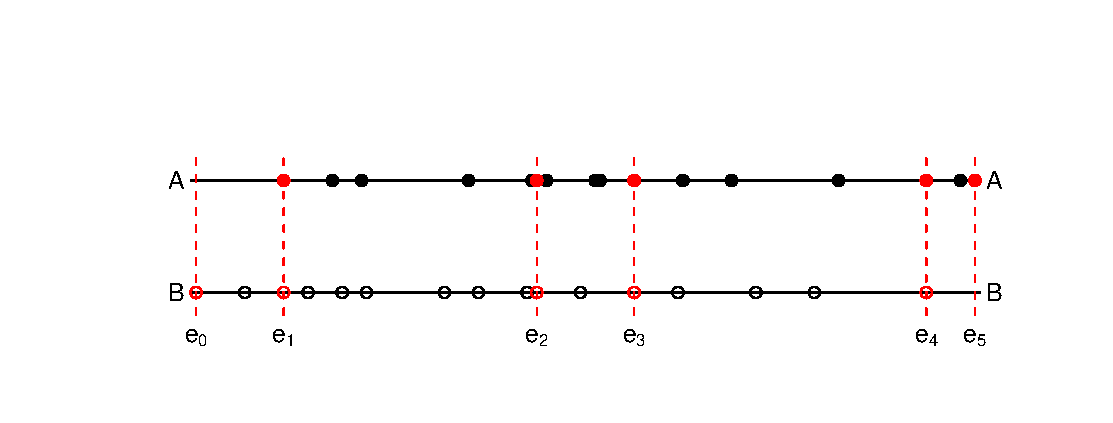
\includegraphics[width=0.95\linewidth]{./Figures/episodes2.eps}
\caption{Times of trades of assets $A$ and $B$.  The points $(e_1,\dots,e_4)$ are synchronisation points. These points separate the process into independent asynchronous episodes. In this illustration, prior to $e_1$ only asset $B$ provides information and after $e_4$ only asset $A$ \label{fig:1}}

\end{figure}

The likelihood can then be written as
$$L(\theta) = L_0^*(\theta) \prod_{k=1}^K L_k(\theta) L_1^*(\theta),$$
where $L_0^*(\theta)$ and $L_1^*(\theta)$ depend on the data from a single asset (at the beginning and end of the sequence) and $L_k(\theta)$ depends on data from the $k$th asynchronous episode. Note that if synchronisation is frequent this produces substantial savings in the cost of calculating the likelihood.

When $L_0^*(\theta)$ depends only on asset $A$, for example, we have
$$L_0^*(\theta) = \frac{\exp\left[ -\frac1{2 \sigma^2_1} \sum_{i=1}^{n_0} r_i^2/\tau_i^X\right]}
{\prod_{i=1}^{n_0}\sqrt{2 \pi \sigma^2_1/\tau_i^X}},$$
where $n_0$ is the number of return periods prior to the first asynchronous episode and $r_i$ is the $i$th return for that asset.

For a typical asynchronous episode we have
$$L_k(\theta) = \frac{\exp\left(-\frac12 \bar{r}^\text{\sf T} V^{-1} \bar{r}\right)}{(2 \pi)^{(m+n)/2}\sqrt{\text{det}(V)}},$$
where $\bar{r}$, $m$, $n$ and $V$ now refer to the information in that episode.  For notational simplicity we will not annotate these terms  with $k$.  

Using \eqref{matrix} we have
$$L_k(\theta) =  \frac{\exp\left(-\frac12(M_1 - 2M_{12} +M_2)\right)}{(2 \pi)^{(m+n)/2}\sqrt{\text{det}(V)}},$$
where 
\begin{align*}M_1 &= r^{\sf T}(D_1^{-1} - \rho^2 F E^{-1} F^{\sf T})r, \\ M_{12} &= \rho r^{\sf  T}F E^{-1} s/(\sigma_{1} \sigma_{2}), \\ 
 M_2 &= s^{\sf T}E^{-1}s/\sigma^2_2,\end{align*}
and the det$(V)$ can be calculated as $\sigma_{1}^{2n} \sigma_{2}^{2m} \text{det}(D_1) \text{det}(D_2 - \rho^2 B^{\sf T} D^{-1}_1 B). $

The combined likelihood then becomes
\begin{equation}\label{likelihood}
L(\theta) = \frac{\exp\left(-\frac12(Q_1(\rho)/\sigma^2_1 - 2Q_{12}(\rho)/(\sigma_{1} \sigma_{2}) +Q_2(\rho)/\sigma^2_2)\right)}{(2 \pi)^{(m+n)/2}\sigma_{1}^{m} \sigma_{2}^{n}\sqrt{v(\rho)}},
\end{equation}
where $v(\rho)$ arises as a product of determinants and $Q_1(\rho)$, $Q_2(\rho)$ and $Q_{12}(\rho)$ are sums of quadratic terms from the components of the partitioned likelihood, depending only on $\rho$. 


\subsection{Profile likelihood for correlation}
Maximising  \eqref{likelihood} with respect to $\sigma^2_1$ and $\sigma^2_2$ for fixed $\rho$ is straightforward.  The maximising values can be given explicitly into terms of $Q_1(\rho)$, $Q_2(\rho)$ and $Q_{12}(\rho)$.  Hence the profile likelihood for $\rho$ can be calculated and confidence intervals for $\rho$ evaluated by considering the values of $\rho$ at which the profile log-likelihood falls significantly below its maximum.
This algorithm has been implemented and applied to data relating the USD-JPY exchange rate and the price of 10 year US treasury bond futures.  The results are not included here.
\subsection{Kalman filter}
As with volatility estimation in Chapter 4 the likelihood can be evaluated by the Kalman filter and then maximised routinely. 
 For large scale problems involving data at multiple time points this is a substantial computational task.  For smaller problems this becomes feasible.  Timing comparisons were made between the partitioning methods described in Section \ref{partitioning} and the Kalman filter using a subset of the USD-JPY exchange rate and 10 year US Treasury bond futures data. The results indicate that the partitioning method is competitive with the Kalman filter when implemented in {\sf R} using the `fast' Kalman filter package. We have not given numerical comparisons here because they are highly sensitive to implementation details.  
\subsection{Recursive covolatility estimation}
It should be noted that maximum likelihood estimation will never be a serious competitor for covolatility estimation in high-speed trading. It is a batch processing algorithm that may be of use in historical analysis.  The advantage of the ZHY estimator and its extensions is that they can be calculated in linear time, linear in the number of data points. Furthermore, we can produce exponentially weighted versions of the estimators that can be updated using simple recursion as described in a more general context in Chapter 3 and specifically for volatility estimation in Chapter 4. This enables changing patterns of covolatility to be monitored in real time.
